% !TEX root = ANA-GENR-2018-01-INT1.tex
% Turn off some chktex warnings.
% chktex-file 1 chktex-file 8 chktex-file 46

%------------------------------------------------------------------------------
\section{ATLAS work strategy}%
\label{sec:ATLAS_work_strategy}
%------------------------------------------------------------------------------

%------------------------------------------------------------------------------
\subsection{ATLAS analyses and publications}%
\label{sec:The_ATLAS_Analyses_and_Publications}

ATLAS experiment supports a  general physics programme to explain the nature of matter. To do so,  it makes use of the gigantic hadron accelerator (LHC), which collides protons at almost the speed of light. With the centre-of-mass energy of \SI{13}{\TeV} provided by the accelerator, we explore matter, its interaction, its properties and simulate small big bangs every second.

To perform such a physics program, physicists need software and graphics tools such as Web and Twiki interfaces to analyse the data and compare them to the different models on the market.
For this, ATLAS is organised in several Physics (PHY) and  Combined Performance (CP) groups and subgroups. These groups are coordinated by conveners, who are elected or appointed by the collaboration for one or more years.
For example, some  PHY and CP groups are label ed top quark (TOPQ), Standard Model (STDM), \PB physics (BPHY), Higgs (HIGG), Electron/Gamma (EGAM), Jet and EtMiss (JETM).
Further studies on system detectors (SYS) or other activities like software (SOFT) and data preparation (DAPR) are also organised hierarchically with subgroups and conveners.

Once an analysis is finished or an aspect of the detector performances has been studied in detail,
the analysis team is asked to prepare a publication.
In fundamental research, as is the case with the research conducted at CERN, the communication to the public is  compulsory and is the only way to demonstrate and show the results.

ATLAS considers three different types of publications:
\begin{itemize}
    \item[\tiny$\bullet$] general publications based on data and the project-related publications (PAPER);
    \item[\tiny$\bullet$] public documents classified as notes (PUB notes);
    \item[\tiny$\bullet$] conference proceedings (PROC) or notes (CONF Notes) on preliminary results, which are shown at conferences.
\end{itemize}

All ATLAS analyses are discussed and presented in the relevant working groups  (physics, combined performance, systems and detectors, etc.). The Physics Coordinator, the working groups conveners and the Publication Committee members are informed of all ongoing analyses and publications. They also appoint analysis contacts, contact editors,review experts and the Editorial Board which is in charge to launch the publication process as described in this \href{https://cds.cern.ch/record/1980862}{Pub note}.

The working groups and subgroups have the responsibility to provide guidance, help and/or resources to the analyses during their early stages and throughout their development. A review of the analysis by the working group takes place throughout the development phase. The working groups should also develop a coherent and realistic plan for the release  of the results for a conference and/or for a journal publication. This is a necessary step before any paper draft can be planned or circulated. The constitution of Analyses groups, the appointments or group and sub group conveners, analysis contacts and the Editorial Board members are done using the\textbf{ Fence/Glance} system which is being is described in section~\ref{sec:The_FENCE_project}. Analyses and Documents are handled through different phases as described in section~\ref{sec:Analysis_and_paper_phases}.

To summarize:
\begin{itemize}

    \item[\tiny$\bullet$]
The launch of an analysis or a document is done at the so-called \textbf{PHASE~0} of the system. PHASE 0 is a special system which is integrated with Gitlab. Consequently, editors can already request repositories to edit any type of document (PAP, CONF, PUB) and as many so INT (internal)  drafts. The Glance-Gitlab system is described in section{}

    \item[\tiny$\bullet$]
    
The Editorial Board (EdBoard) reviews the complete analysis and ensures that both the supporting documentation and the paper draft are well prepared. Members of the EdBoard are requested to inspect tables and plots, scrutinise the background determination procedures and systematic uncertainty evaluations, and critically examine the result extraction. The EdBoard is required to sign off on the supporting documentation (analysis) and draft paper or CONF note before its circulation to ATLAS. The EdBoard should verify that the analysis is worth publishing in the proposed form, and consult with the PubComm (Publications Committee) chair if there are doubts. It should also establish with the editors and conveners whether the paper should be a letter or an article, and propose a journal. These tasks and validation steps are translated as validation workflow in Fence/Glance system in theirs \textbf{PHASE~1} and \textbf{PHASE~2}, related respectively to the 1st and 2nd circulation to the collaboration, two sequences of the process of a validation of a publication.

All signing authors of the ATLAS collaboration are expected to read and comment on paper and/or note drafts.

    \item[\tiny$\bullet$]

The Publication Committee (PubComm) chair has the responsibility to assess the quality of the paper and to ensure ATLAS guidelines and policies are followed. After the Public Reading, and the sign-off by the EdBoard of a draft  that addresses all comments made to draft-1 (PHASE~1) and draft-2 (PHASE~2)  and at the Public Reading, the draft goes to the chair of PubComm for a final sign-off.

    \item[\tiny$\bullet$]

The Spokesperson is ultimately responsible for the scientific quality of the results from the ATLAS collaboration and has a final look at each paper before the \textbf{submission}. The Final draft  is signed-off by the spokesperson or its delegate. 

    \item[\tiny$\bullet$]
    
As soon as the SP has signed-off, the validation workflow at Phase 2 is finished and send a message to the Physics Office Publications crew to announce them an expected submission. PO-PUB officers use the \textbf{SUBMISSION} phase of the system and proceed with the submission to arXiv and the Journal reviews as well as all the necessary communication steps with the journal through a dedicated validation workflow until the final publication.

\end{itemize}

For the CONF or PUB notes there are no PubComm or Spokesperson reviewers. Instead the Physics Coordinator appoints two members of the collaboration to review the draft and perform the final sign-off. These two types of documents need only PHASE~1.


%------------------------------------------------------------------------------
\subsection{Author lists, Acknowledgments and Proof Checker}%
\label{sec:Authorlists_acknowledgments_and_ProofChecker}

Author lists and Acknowledgements are two of the final steps of a paper’s publication and both are handled and generated, using the FENCE framework, described in detail in \cref{sec:The_FENCE_project}.
After the papers containing the author lists and acknowledgements are submitted to the journals,
they come back to the ATLAS Physics Office for a final review before the publication.
This review is mainly performed automatically using a PO tool: the Proof Checker.

The author list is the inventory of qualified authors at a given date, which is also called the reference date. Every paper has a related list of qualified authors with a reference date which corresponds to the creation date of that list at the Paper Phase 1, just before the first circulation to the collaboration. Qualified authors are active physicists, still contributing to the maintenance and the operations of the collaboration.
Some of them are retired people benefiting from their pre-data credits (worked before the data era), called signing-only authors.
Between FENCE PHASE~1 and PHASE~2, some people may get exceptional authorship because of their involvement in the analysis or the paper,
even if they are not yet a qualified author.
Therefore the author list is updated to include \enquote{exception} authors.The special cases are studied by the Authorship Committee and proposed for approval to the Spokesperson who will agree or not for this exception after reviewing the proposal from the authorship committee.

All this information is stored in the ATLAS database and managed by FENCE\@.
\Cref{fig:authorlist_generation} shows a the start of the full list of members (active and retired), their institutes and the related metadata that is needed to generate a full report of members and institutes.

\begin{figure}[htb]
  \centering
  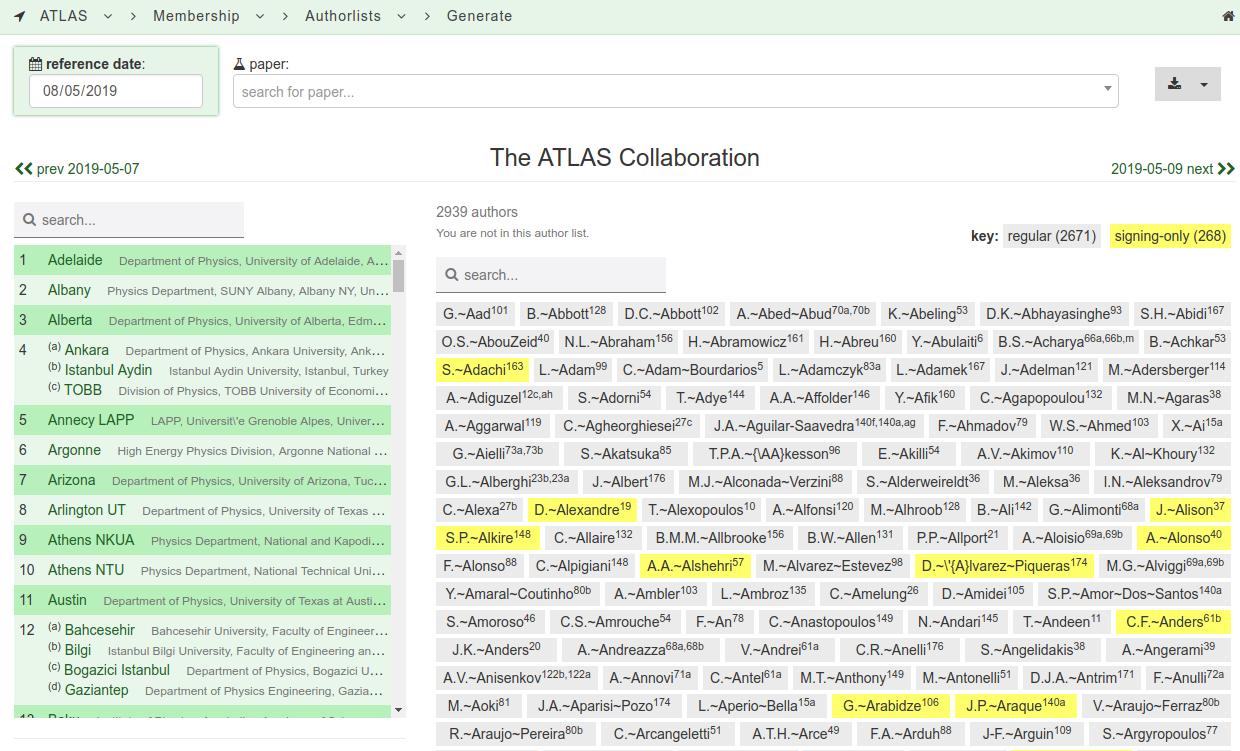
\includegraphics[width=0.9\textwidth]{figures/authorlist_generation.png}
  \caption{FENCE author list generation interface.
    \GSnote[inline]{}{Please expand the caption more to include explanation of the different piecces of the screen. Why are some names yellow? What's the green stuff on the left? Who can access this interface?}}%
  \label{fig:authorlist_generation}
\end{figure}

The acknowledgements are a legal paragraph that the collaboration agrees to add in each paper to thank for their financial support.
They do not change very often, but may include or suppress a Funding Agency or Foundation at a given date.
Therefore, an acknowledgement file is built for each paper at a specific date, which is called the reference date.

The proof checker is a tool provided mainly for the ATLAS PO members to compare the final publication (PDF file) of author lists and acknowledgement provided by the journal with ATLAS data (XML file). The main purpose of the proof checker is to identify inconsistencies between data provided to the journal and what the journal will produce as final output. A report of this comparison, one for every version of the proof, is available to the ATLAS PO members so they can check the results.

\GSnote{}{Expand more on proof checker? Shouldn't you have three subsections here? One discussing the FENCE interface for author lists, one that discusses more about how the acknowledgements are generated -- explaining that they're reviewed by a legal team if at all, and more about how that's generated; and more about the proof checker. Is it a script? How is it almost fully-automated? Does someone run it or is it automatically run? What's the example output, etc...?}
